\scanpage{17}
\mspage{16}
\mspage{IV-962}

que de $k$ ; il est alors immédiat que $K\otimes_k\Omega$ est composé direct d'un nombre fini de corps, tous isomorphes à la clôture séparable $K\Omega$ de $K$. D'autre part, l'anneau ${}^{\mathrm{hs}}A$ étant hensélien, $C\otimes_A({}^{\mathrm{hs}}A)$ est composé direct des anneaux locaux $(C\otimes_A({}^{\mathrm{hs}}A))_{\underline{q_{\unsure{1|i}}}}$, où $\underline{q_{\unsure{1|i}}}$ $(1\leq\unsure{1|i}\leq s)$ parcourt les idéaux maximaux de \deleted{$\unsure{C'}$} $C\otimes_A({}^{\mathrm{hs}}A)$, et ces anneaux locaux sont henséliens (18.5.10) et ont $K\Omega$ pour corps résiduel, donc sont strictement locaux (18.8.1). Posons pour abréger $C'=C\otimes_A({}^{\mathrm{hs}}A)$ et $C_{\unsure{1|i}}'=C'_{\underline{q_{\unsure{1|i}}}}$, qui est donc un anneau quotient de $C'$ ; soient $f:C\to C'$, $g:{}^{\mathrm{hs}}A\to C'$, $\varphi_{\unsure{1|i}}:C'\to C_{\unsure{1|i}}'$ les applications canoniques.

\diagram{\begin{tikzcd}[column sep=small,row sep=large]
C \arrow[r,"f"'] \arrow[rrr,bend left=22,"v"] & C' \arrow[r] & C_i' \arrow[r,shift right=.65ex,"w"'] & {}^{\mathrm{hs}}C \arrow[l,shift right=.65ex,"w'"'] \\
A \arrow[u] \arrow[r,"\unsure{\prime}"] & {}^{\mathrm{hs}}A \arrow[u,no head] \arrow[urr,"u"'] & &
\end{tikzcd}}

Soit $v:$ \deleted{$\unsure{C\to C'}$} \inserted{$C\to{}^{\mathrm{hs}}C$} l'homomorphisme canonique ; il existe \deleted{\unsure{d'abord}} un homomorphisme local et un seul $u:{}^{\mathrm{hs}}A\to{}^{\mathrm{hs}}C$ qui, par passage aux quotients, donne l'injection canonique $\Omega\to K\Omega$ \deleted{\unsure{(18.8.5)}} et tel que le composé $A\to C\xrightarrow{v}{}^{\mathrm{hs}}C$ soit égal au composé $A\to{}^{\mathrm{hs}}A\xrightarrow{u}{}^{\mathrm{hs}}C$ (18.8.5) ; donc il existe un unique homomorphisme local $w_0:C'\to{}^{\mathrm{hs}}C$ tel que $w_0\circ g=u$, $w_0\circ f=v$, et puisque ${}^{\mathrm{hs}}C$ est un anneau local, cet homomorphisme se factorise en $C'\xrightarrow{\varphi_i}C_{\unsure{1|i}}'\xrightarrow{w}{}^{\mathrm{hs}}C$ pour un indice $\unsure{1|i}$ bien déterminé, $w$ étant un homomorphisme local. D'autre part, l'anneau $C_{\unsure{1|i}}'$ étant strictement local, il existe un homomorphisme local $w':{}^{\mathrm{hs}}C\to C_{\unsure{1|i}}'$ qui, par passage aux quotients, donne l'automorphisme identique de $K\Omega$ et qui est tel que $w'\circ v=\varphi_{\unsure{1|i}}\circ f$ \deleted{\unsure{,}} \inserted{(18.8.5)}. On déduit d'abord de là que $w\circ w'$ est un endomorphisme de ${}^{\mathrm{hs}}C$ qui, par passage aux quotients \deleted{\unsure{à}}, donne l'automorphisme identique de $K\Omega$, donc est l'identité (18.8.5). D'autre part, , on a $w'\circ w\circ\varphi_{\unsure{1|i}}\circ f=w'\circ v=\varphi_{\unsure{1|i}}\circ f$, et $w'\circ w\circ\varphi_{\unsure{1|i}}\circ g=w'\circ u=\varphi_{\unsure{1|i}}\circ g$ ; d'où $w'\circ w\circ\varphi_{\unsure{1|i}}=\varphi_{\unsure{1|i}}$, autrement dit $w'\circ w$ est l'automorphisme identique de $C_{\unsure{1|i}}'$. CQFD.

\uline{Remarque} (18.\unsure{8|9}.\deleted{7}\inserted{10}.1).-- La démonstration de (18.8.7) n'utilise le fait que $B$ est une $A$-algèbre finie, que pour établir que $K\otimes_k\Omega$ est composé direct d'un nombre fini de corps. Or, cette dernière propriété est encore vérifiée lorsque l'on suppose que $B$ est une $A$-algèbre \uline{entière semi-locale} dont les idéaux maximaux $\underline{n_j}$ ont des corps résiduels de degrés séparables $[\kappa(\underline{n_j}):k]_s$ \uline{finis}.
\margin{\figure{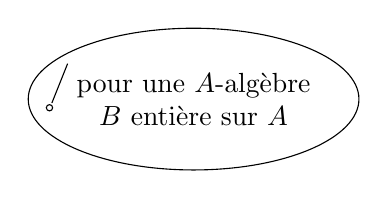
\begin{tikzpicture}\draw (0,0) ellipse (2.1 and .9);\node[align=center] at (0,0) {pour une $A$-algèbre\\$B$ \uline{entière} sur $A$};\draw (-1.8,-.05)--(-1.6,.45);\draw (-1.83,-.11) circle (.04);\end{tikzpicture}}}

\uline{Proposition} (18.8.\deleted{8}\inserted{11}).-- \uline{Soit} $A$ \uline{un anneau} \deleted{\unsure{noethérien}} \uline{semi-local}.

(i) \uline{Pour que} ${}^{\mathrm{hs}}A$ \uline{soit réduit} (resp. \uline{normal), il faut et il suffit que} $A$ \uline{le soit}.

(ii) \uline{Supposons} $A$ \uline{noethérien. Alors, pour tout idéal premier} $\underline p$ \uline{de} $A$, \uline{l'anneau} $({}^{\mathrm{hs}}A)_{\underline p}/\underline p\cdot({}^{\mathrm{hs}}A)_{\underline p}$ \uline{est composé direct d'un nombre fini d'extensions algé-}

